\documentclass{article}

\usepackage[english]{babel}
\usepackage[margin=3cm]{geometry}
\usepackage{graphicx}
\usepackage{float}
\usepackage{caption}
\usepackage{hyperref}
\usepackage{amsmath}
\usepackage{wrapfig}
\usepackage[parfill]{parskip}

% fonts
\usepackage[T1]{fontenc}
\usepackage{helvet}
\renewcommand{\familydefault}{\sfdefault}

\graphicspath{{img/}}

% theorem environment
\usepackage{amssymb}

\newtheorem{theorem}{Definition}[section]

\usepackage{enumitem}

\newenvironment{thmenum}
 {\begin{enumerate}[label=\upshape\bfseries(\roman*)]}
 {\end{enumerate}}


% code
\usepackage{minted}
\setminted{frame=single,framesep=3pt,linenos}
\usepackage{upquote}
\usepackage{color}

\begin{document}

\begin{titlepage}
    \author{Tuur Vanhoutte}
    \title{MLOps}
\end{titlepage}

\pagenumbering{gobble}
\maketitle
\newpage
\tableofcontents
\newpage

\pagenumbering{arabic}

\section{Introduction}

\begin{itemize}
    \item Deployment of deep learning models in an API
    \item Deploying services to Kubernetes with Docker
    \item Version Controlling with Git (to blame those who ruined the code)
    \item Automation pipelines to prepare data, train models and deploy applications
    \begin{itemize}
        \item Automated delivery (ready to deploy)
        \item Automated deployment (CI / CD)
    \end{itemize}
\end{itemize}

\subsection{Why do I need deployment automation}

\begin{itemize}
    \item Save time
    \item Increased accuracy
    \item Better documentation
    \item Autoscaling
\end{itemize}

\subsection{What will we do}

\begin{itemize}
    \item Object classification with a CNN
    \item Deployed with FastAPI 
    \item Scalable with Kubernetes
    \item Automated with CI/CD pipelines
    \begin{itemize}
        \item Yes, also automated AI Training!
    \end{itemize}
\end{itemize}


\subsection{The AI pipeline}

\begin{figure}[H]
    \centering
    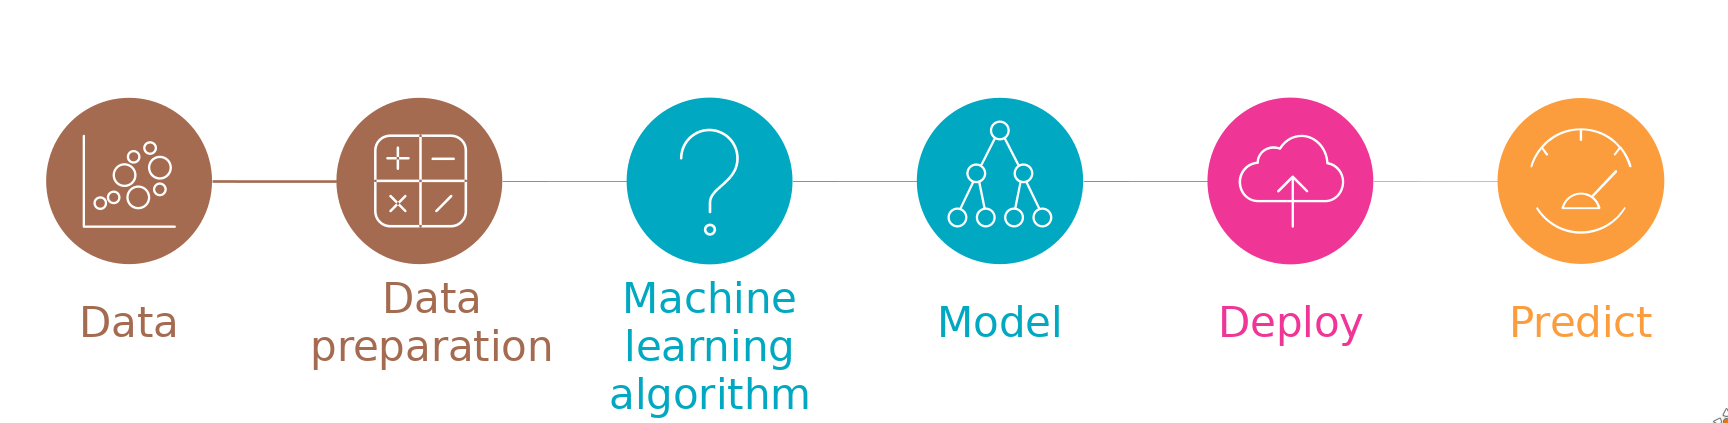
\includegraphics[width=0.8\textwidth]{complete-pipeline.png}
    \caption{The complete AI pipeline}
\end{figure}

\subsection{Teleport}

How to connect to your dedicated virtual machine? 
\textbf{Teleport} allows engineers and security professionals 
to unify access for SSH servers, Kubernetes clusters, 
web applications, and databases across all environments.

\subsubsection{Teleport Server Access}

\begin{itemize}
    \item One centralized login and user-management system
    \item Randomly generated passwords for your user account
    \item We manage all virtual machines your use can access
\end{itemize}

To \textbf{install and use Teleport}, see Leho.

\section{FastAPI}

TODO

\section{Docker}

TODO

\end{document}